% Charlotte Geiger - Manuel Lippert - Leonard Schatt
% Physikalisches Praktikum

% Teilaufgabe X

\section{Vorbereitung für den Versuchsaufbau}

\begin{figure}[h]
    \begin{center}
        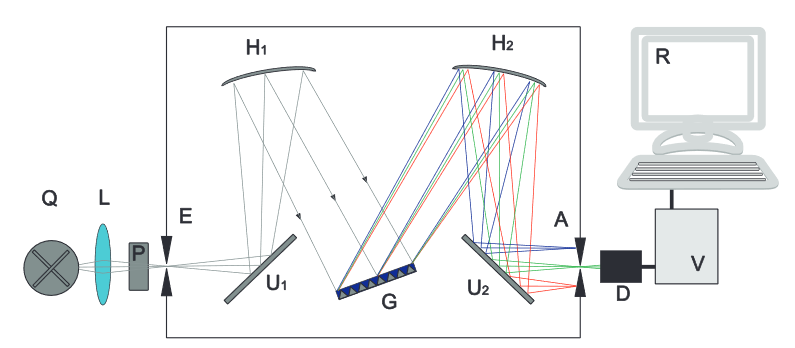
\includegraphics[width=10cm]{Bilder/SP1.PNG}
    \end{center}
    \caption{Versuchsaufbau}
    %\label{fig:meine-grafik}
\end{figure}
Die Sammellinse und der Eintrittsspalt müssen nach der Abbildungsgleichung 
\begin{equation}
    \frac{1}{f}= \frac{1}{g}+\frac{1}{b}   
\end{equation}
In der Abbildungsgleichung bezeichnet $b$ den Abstand vom Bild zur Linse und $g$ den Abstand vom Gegenstand zur Linse. $f$ ist die Brennweite. Setze jetzt $b = g $, also der Abstand zwischen 
Lampe, Bild und Spalt sollte gleich sein. So schafft man eine 1:1 Abbildung. 
\begin{equation}
    \frac{1}{f} = (\frac{1}{b}+\frac{1}{b})^{-1} = (\frac{1}{g}+\frac{1}{g})^{-1}
    \newline
    \Rightarrow g = b = 2f
\end{equation}
ist dies der Fall. Die Sammellinse sollte also um $b$ vom Eintrittsspaltentfernt sein.\\
Der Hohlspiegel fungiert in diesem Aufbau wie eine Linse. Damit die Strahlen, welche über einen Spiegel umgeleitet werden, nach dem Spiegel parallel liegen, muss der Eintrittsspalt genau in der Brenneben liegen. Der Abstand zwischen Eintrittsspalt und Hohlspiegel muss also $f_{Spiegel}$ sein.\\
Beim zweiten Spiegel ist die Argumentation die Selbe, nur in die andere Richtung. Deswegen ist der Abstand zwischen Hohlspiegel und Austrittsspalt $f_{Spiegel}$.